% IN4387: System Validation project
% MAIN FILE

% PLEASE NOTE: DO NOT EDIT THIS FILE !! Always make sure that the report is buildable at all times. Nothing is more annoying than having changed something but being unable to see the result because someone else has been messing around. YOU SHOULD ALWAYS WORK IN A LOCAL WORKING DIRECTORY AND ONLY SHARE FILES ONCE THEY BUILD CORRECTLY. Shyam will eat you alive if you don't do this, you have been warned!!

\documentclass[11pt,a4paper]{report}

% Save some trees...
\setlength{\topmargin}{-1.3cm}
\setlength{\textheight}{24cm}
\setlength{\oddsidemargin}{0cm}
\setlength{\textwidth}{15.9cm}
\linespread{1.0}

% Packages
\usepackage[english]{babel}
\usepackage{listings}
\usepackage{graphicx} \graphicspath{{./figures/}}
\usepackage{url}
\usepackage{algorithm}
\usepackage[noend]{algorithmic}
\usepackage{clrscode}
\usepackage{caption}
\usepackage{subcaption}
%\usepackage{subeqn}
\usepackage{amsmath}
%\usepackage[nottoc,numbib]{tocbibind}

%special auto table
%\usepackage{tabularx}

\usepackage[parfill]{parskip}
% package for euro symbol
\usepackage{eurosym}
% Some helping commands
\newcommand{\figref}[1]{Figure \ref{#1}}
\newcommand{\vect}[1]{\textit{\textbf{#1}}}
%Use package for hyperlink
\usepackage{hyperref}
\begin{document}
\selectlanguage{english}
\title{IN4387 System Validation\\
		\textbf{Design \& Verification of Controller for a Package Storage System}}
\author{S. Balasubramanian, \#0785610\\
			Voudouris. P, \#0788565\\
			Gozek. E, \#0786244\\\\
Eindhoven University of Technology\\
Department of Embedded Systems}
\maketitle

\tableofcontents

% These chapters are already put into separate files

%\chapter{EXAMPLES}
%\label{chap:examples}
%\section{A section}
\label{sec:exampleA}

You can see a random figure in Figure \ref{fig:googlelogo}.

A list:
\begin{itemize}
\item An item
\item And another one
\end{itemize}

\begin{figure}[h]
\center

\includegraphics[width=0.6\textwidth]{google}
\caption{This is the google logo}
\label{fig:googlelogo}
\end{figure}


An example of a table is given in table \ref{tab:randomtable}. See the literature list at the end of the report somewhere.

\begin{table}[h]
\center
\begin{tabular}{|l|c|}\hline
left aligned column & centred column \\\hline
next row  & random content\\\hline
\end{tabular}
\caption{This table contains stuff}
\label{tab:randomtable}
\end{table}

This is an example of a reference \cite{becker}.

And here a new example: pseudocode \ref{algo:dfs}!
\begin{algorithm}
\caption{\proc{DepthFirstSearch}}
\label{algo:dfs}
\begin{algorithmic}[1]
\REQUIRE A graph $G=(V,E)$ in adjacency list presentation, starting vertex $v$, an empty stack $S$
\ENSURE All vertices in this connected component labelled
\STATE label $v$
\STATE push all neighbours of $v$ on $S$
\WHILE{$S$ \NOT empty}
	\STATE $w \leftarrow$ pop $S$
	\STATE label $w$
	\FOR{$u$ in adjacency list $w$}
		\IF{$u$ \NOT labelled}
			\STATE push $u$ onto $S$
		\ENDIF
	\ENDFOR
\ENDWHILE
\end{algorithmic}
\end{algorithm}


\section{Another section}
You should read all the stuff in section \ref{sec:exampleA}. This section holds only an example of a reference ;)


%\chapter{Introduction}
%\label{chap:introduction}
%% Introduction to what a Packet storage is. Discuss its strcuture.
% Where is it used, and how is it useful.
% How many controllers it has (and why)
% What is in the report (section-wise)

The project described in this report discusses the design and verification of a small packet storage system. The packet storage system is inspired by the distributed controller of an operational product manufactured by Vanderlande, a Dutch company. 
The aim of this project is to understand and formulate the requirements of such a system, design the system and in the end verify that the system would meet the proposed requirements when in operation under any circumstance.

The packet storage system consists of two conveyor belts, one for receiving a packet into the system and the other for delivering the packet out of the system. The system consists of several racks where packets can be stored. The packets are stored by means of two elevator platforms (situated serially, one above the other). Moreover, there are five controllers in the system which run in parallel. Figure \ref{fig:packet_storage} shows the diagram of such a system. The controller C1 controls the input conveyor belt, controller C2 controls the output conveyor belt, conveyor C3 and C4 operate its respective elevators and controller C5 keeps track of all the information about racks, packet storage and its dispatch.

\begin{figure}[h]
\center
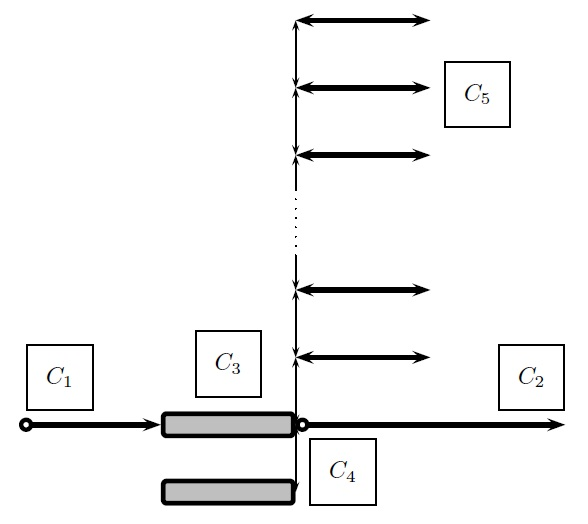
\includegraphics[width=0.6\textwidth]{packet_storage_diag}
\caption{Packet storage system, courtesy \cite{problem_statement}}
\label{fig:packet_storage}
\end{figure}

There are however, certain constraints to be understood for the given system. For example, the number of packets on the conveyor belt, rack slots and elevator platform can carry only one packet at a time, etc. Further constraints are discussed in the next section under global requirements.

The sections described in the report are the global requirements, external interactions in the system, translated requirements, the architecture of the system transpired, discussion on controllers with its labelled transition diagram(LTS) and finally discuss the verification of its global requirements.
The system is to be modelled to be intelligent to fulfil the basic requirements desired from such a system.

\chapter{Global requirements}
\label{chap:globalrequirements}
\section*{Global Requirements}
\label{sec:global_req}
In this chapter, we list the global requirements essential for the design of the controller:
\begin{enumerate}
\item Each elevator, rack and conveyor belt contains at most one packet.
\item Packet is exchanged only when the elevator platform is at the same level as that of a conveyor belt.
\item Packet is exchanged only when elevator platform is at the same level as that of a rack.
\item The two elevators cannot be at the same position.
\item The lower elevator must never pass the upper one.
\item Packets are always delivered in the same order as requested.
\item If a packet is ready to enter and there is a free position at the rack(s), it will be eventually accepted.
\item If a requested packet is in the system, it will be eventually delivered. %unless the system shuts down
\item If a packet is unable to be located, an alarm must be generated.
\item The number of packets in the system can at most be equal to the number of racks.
 
%\item If the input conveyor malfunctions, the remaining packets inside the system must be able to leave, eventually.

%\item \textbf{How:} It should be always possible to know the number of packets in the system.(design decision we will confirm this one after we have decided about working mechanism of our system.)

%\item \textbf{Assumption:} Lower elevator cannot reach the lowest rack and highest elevator cannot reach the highest rack.(remove this one.Since it is included in 4, we do not need to state it again.)

\end{enumerate}

\chapter{System interactions} %what are all the interactions
\label{chap:externalIntr}
% External requirements table with actions/ variables/ sync_comm.
\label{sec:ext_interactions}
This section lists the external and internal interactions for the packet storage system. These are the actions that are essential for the design of the system. The following describe in brief the external and internal interactions used in the system; the action, it parameters and its description.

\subsection*{External Interactions} The external interactions are listed under table \ref{tab: extr_interactions}. These actions are visible to the outside world or the user controlling the system.

\begin{itemize}
\item \textbf{WantIn(id: packetID)}
Environment requires a packet with packet id packetID to be inserted to the system. This is action is managed by controller C1.

\item \textbf{AcceptPacket(id: packetID)}
Controller C1 initiates the AcceptPacket action in order to accept the packet and put it on the conveyor.

\item \textbf{RejectPacket(id: packetID)}
This action is executed by controller C1 in order to inform the user that the packet with \textit{packedID} has not been inserted into the system.

\item \textbf{MoveElevator(eId: elevID,p: pos)}
Controllers C3 and C4 initiate the moveElevator action to instruct the real hardware to move the elevator to the target position $p$.

\item \textbf{WantOut(id: packeID)}
User requests the packet with packet with an $id$ to be delivered by the system. This action is initiated by controller C2.

\item \textbf{PacketNotFound(id: packetID)}
Controller C2 informs the user that the packet with a give $id$ was not found.

\item \textbf{DeliverPacket(id: packetID)}
Controller C2 initiates DeliverPacket action to deliver the packet with an $id$.

\item \textbf{ConvInToElev(eId: elevID)}
With this action, controller C1 instructs the real hardware to transfer the packet from input conveyor to the required elevator.

\item \textbf{ConvInToElev(eId: elevID)}
Controllers C3 or C4 instruct its hardware to transfer the packet from the elevator platform to the rack.
Note: We assume that elevator platform and a rack would have the same position during any exchange.

\item \textbf{RackToElev(eId: elevID)}
Controller C5 instructs the hardware to transfer the packet from rack to the required elevator.

\item \textbf{ElevToConvOut(eId: elevID)}
Controllers C3 or C4 instructs its hardware to transfer the packet from the required elevator platform to the output conveyor.
%What will happen if we give the elevID to be 1.. it would deadlock?%

\item \textbf{GetPosition (eId: elevID, p: pos)}
Get the position $p$ of an elevator with an identifier $id$.

\end{itemize}

\subsection*{Internal interactions}
The internal interactions are listed under table \ref{tab: int_interactions}. These actions are hidden to the outside world or the user controlling the system and take place as interactions within/between individual controllers.

\begin{itemize}
\item \textbf{queryRackSpace(b: bool)}
Queries if a position is available in racks. This is an internal action that is initiated by controller C1.
%Should it be a communication??%

\item \textbf{commPacketOnConveyor(id: packetID, cId: convID)}
This is a synchronizing action whereby controller C1 informs C5 of the packet on conveyor. This action is completed with the acknowledgement from controller C5.

\item \textbf{commOrderMoveElevator(e:ElevID, p: pos)}
Controller C5 synchronizes with an elevator controller (C3/C4) to move it to a target position $p$.

\item \textbf{commAckElevatorMoved(b: bool)}
Elevator controller acknowledges controller C5 of the completion of elevator movement.

\item \textbf{commConveyorToElev(eId: elevID, cId: convID)}
Controller C5 informs C1 to move the conveyor belt and exchange the packet with the elevator with a given $elevID$.

\item \textbf{commPacketOnElevAck(id: packetID)}
Elevator controllers acknowledge controller C5 once packet is received by the elevator.

\item \textbf{commElevToRack(eId: elevID)}
Controller C5 communicates with elevator controllers in order to load to packet to the rack.

\item \textbf{commPacketLoadedToRack(id: packetID)}
Elevator controllers inform C5 that loading of the packet to the rack action is completed.

\item \textbf{commRequestPacket(id: packetID)}
A synchronization action between controllers C2 and C5 to request a packet with a given $id$.

\item \textbf{commPacketExists(b: bool)}
Synchronization action that governs the knowledge of the packet availability from rack controller C5 to C1.

\item \textbf{commRackToElev(eId:  elevID)}
This action governs the communication of reception of packet from conveyor belt.

\item \textbf{commElevToConveyor(eId: ElevID)}
This action governs the communication of unloading a packet to the conveyor belt.

\item \textbf{commElevToRack(eId: elevID)}
Elevator communication with controller C5 after an outgoing transaction is complete.
\end{itemize}

\subsection*{External Interactions}


\subsection*{Data types}
The data types used are described in table \ref{tab: data_types}.
\begin{table}[ht]
\centering
\begin{tabular}{|l|l|l|}\hline
Datatype & OfType & Range$\slash$Members\\\hline
packetID & $Nat+$ & {1..N} \\\hline
elevID & $Nat+$ & {1, 2}\\\hline
pos & $Int$ & {-1..N}\\\hline
b & $bool$ & {true, false} \\\hline
\end{tabular}
\caption{Data types in our design: Packet storage system }
\label{tab: data_types}
\end{table}


%
%
%\begin{table}[ht]
%\centering
%\begin{tabular}{|l|l|l|}\hline
%Action & Description & Parameter \\\hline
%WantIn & Environment requires a packet to be inserted & packetID \\\hline
%QueryRackSpace & Queries if a position is available in racks & bool \\\hline
%AcceptPacket & Accept the packet and put it on the conveyor & packetID \\\hline
%commPacketOnConveyor & Informs C5 of the packet on conveyor & packetID \\\hline 
%commOrderMoveElevator & Order elevator to go to a target position & elevID, pos \\\hline
%commAckElevatorMoved & Acknowledge C5 of the completion of elevator movement & bool: b \\\hline
%MoveElevator & Move elevator hardware to a target position & elevID, pos \\\hline
%commConveyorToElev & Transfer packet to conveyor & elevId \\\hline
%commPacketOnElevAck & Acknowledge C5 once packet is received by elevator \\\hline
%commElevToRack  & Communication of load of packet to conveyor\\\hline
%WantOut & User requests a packet to the system & packetID \\\hline
%commRequestPacket & Request packet to C5 & packetID \\\hline
%commPacketExists & Information provided by C5 to C2 of availability \\\hline
%PacketNotFound & Inform user that the packet is not found \\\hline
%commRackToElev & Communication of reception of packet from conveyor \\\hline
%commElevToConveyor & Communication of unloading a packet to conveyor \\\hline
%commElevToRack & Elevator communication with C5 after an outgoing transaction \\\hline
%DeliverPacket & Delivers the requested packet to user & packetID \\\hline
%\end{tabular}
%\caption{External interactions: Packet storage system }
%\label{tab: ext_interactions}
%\end{table}

\chapter{Translated requirements}
\label{chap:translateReq}
%Lists all the translated global requirements
% This must cover all possible scenario for each of the global requirements that we decided.
% I have tried to list out all possiblities (in a way that modal-u-calculus) can be written for these translations (sounding negative is important to formulate modal formula much easily). Refer to the report from last year. Feel free to include anything that I may have missed out. (Leave a comment also so that we are aware what changed)

This section lists the requirements from section \ref{sec:global_req} in terms of interactions described in section \ref{sec:ext_interactions}.

\begin{enumerate}
\item \textit{Each elevator, rack and conveyor belt contains at most one packet}

	\textit{Conveyor Belt}
	\begin{itemize}
	\item
	Whenever an AcceptPacket(id: packetID) action is performed it
	is not possible to perform another AcceptPacket(id:
	packetId) unless a ConvToElevator(e: elevID) action is
	performed in the meanwhile (where, e can be one of the two elevators)
	\item Whenever ElevToConvOut(e: elevID) action is performed it is
	not possible to perform another ElevToConvOut(e: 
	elevID) unless a DeliverPacket(id: packetID) action is performed in the meanwhile.
	\end{itemize}
	\textit{Elevator}
	\begin{itemize}
	\item Whenever a ConvToElev(e: elevID) or RackToElev(e: elevID) 
	action is performed it is not possible to perform another
	ConvToElev(e: elevID) or RackToElev(e: elevID) unless an 
	ElevToRack(e: elevID) or ElevToConv(e: elevID) action is performed.
	\end{itemize}
	
	\textit{Rack}
	\begin{itemize}
	\item Whenever an ElevToRack(p: pos, r: rackID) action is done it is not
	possible to perform another ElevToRack(p: pos, r: rackID) unless a RackToElev(p: pos, r: rackID) action is performed.%What about ConvToElev() missing?
	\end{itemize}

\item \textit{ Packet is exchanged only when the elevator platform is at
the same level as that of a conveyor belt}
	\begin{itemize}
	\item Whenever a ConvInToElev(e: elevID) or a ElevToConvOut(e: 
	elevID) is done a MoveElevator(e :elevId, 0: pos) must be
	performed before, without any successor MoveElevator(e :elevId, p: pos) action in the meanwhile where p is a position different than 0.\\(Assumption: Input and output conveyor are at
	position zero.).	
	\end{itemize}

\item \textit{Packet is exchanged only when elevator platform is at the same level as that of a rack}
	\begin{itemize}
	\item ElevToRack(e: elevID, r: rackID) action can only be performed after
	MoveElevator(e: elevID, p: pos) action.
	\end{itemize}
	
\item \textit{The two elevators cannot be at the same position}
	\begin{itemize}
	\item If there is a last action from type MoveElevator(e: elevID, p: pos),
	there cannot be a MoveElevator(e': elevID, p: pos) action unless 
	MoveElevator(e: elevID, p': pos) action takes place.

	\end{itemize}
		
\item \textit{The lower elevator must never pass the upper one}
	\begin{itemize}
	\item Controller C4 cannot initiate the MoveElevator(e: elevID, p: pos) 
	action if the last type of action of controller C3 is MoveElevator(e': elevID, p': pos).\\
	\textit{Note:} Here, p $>$ p' and e, e' is the lower and 
	upper elevator, respectively. We assume C4 controller to control
	the lower elevator and C3 controls the upper elevator.
	\end{itemize}
	
\item \textit{Packets are always delivered in the same order as
	requested}	
	\begin{itemize}
	\item 
	For all WantOut($id$: packetID) and a following WantOut($id'$: 
	packetID) \textit{a DeliverPacket(id: packetID) in the meanwhile} it
	should be never be possible to perform DeliverPacket($id'$: 
	packetID) followed by DeliverPacket($id$: packetID).
	\end{itemize}
	
\item \textit{If a packet is ready to enter and there is a free
	position at the rack(s), it will be eventually accepted}
	\begin{itemize}
	\item Whenever the difference in the number of 'AcceptPacket'
	actions and number of 'DeliverPacket' actions is  smaller than the
	number of racks in the system, a new AcceptPacket(id: packetID)
	action should be possible.
	\end{itemize}
	
\item \textit{If a requested packet is in the system, it will be
	eventually delivered}
	\begin{itemize}
	\item When a WantOut(id: packetID) appears after an AcceptPacket(id: 
	packetID) then eventually a DeliverPacket(id: packetID) must be
	performed.  
	\end{itemize}
	
\item \textit{If a packet is unable to be located, an alarm must 
	be generated}
	\begin{itemize}	
	\item  Whenever a WantOut(id: packetID) action is performed after an 
	AcceptPacket(id: packetID) action, an alarm must be generated if a 
	DeliverPacket(id: packetID) action is not performed.
	\end{itemize}
		
\item \textit{The number of packets in the system can at most be equal to the number of racks}
	\begin{itemize}
	\item The difference in the number of 'AcceptPacket'
	actions and number of 'DeliverPacket' actions can at most be 
	equal to the number of racks in the system.
	\end{itemize}
\end{enumerate}
%End of translations.

\chapter{Architecture} %The main block diagram
\label{chap:architecture}
\section*{Architecture of Packet storage system}

\begin{figure}[h]
\center
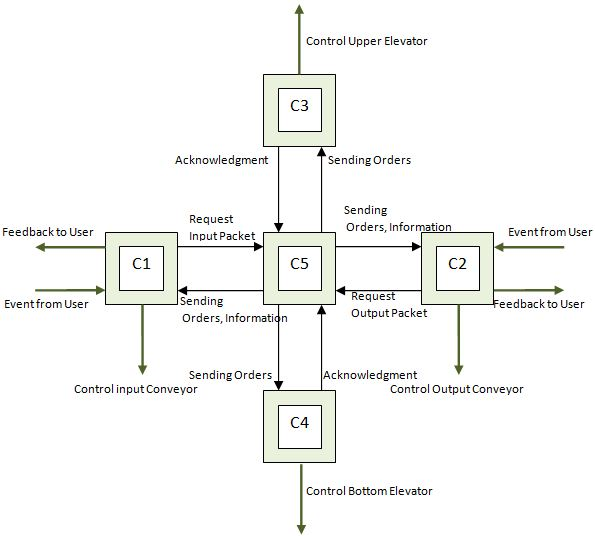
\includegraphics[width=0.7\textwidth]{Architecture}
\caption{Architecture of the system}
\label{fig:architecture}
\end{figure}

%\chapter{Modelling the controller}
%\label{chap:modelController}
%\subsection*{Controller C1}
\begin{figure}[h]
\center
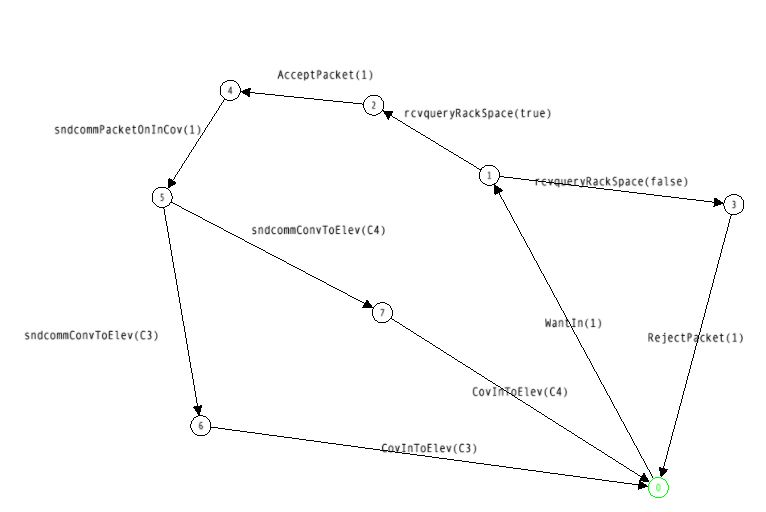
\includegraphics[width=0.7\textwidth]{model_C1}
\caption{Architecture of the system}
\label{fig:controller_C1}
\end{figure}



\subsection*{Controller C2}
\begin{figure}[h]
\center
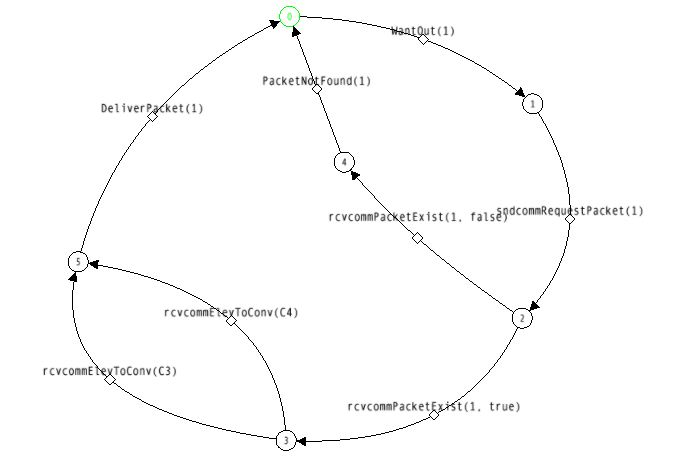
\includegraphics[width=0.7\textwidth]{model_C2}
\caption{Architecture of the system}
\label{fig:controller_C2}
\end{figure}



\subsection*{Controller C3/C4}
\begin{figure}[h]
\center
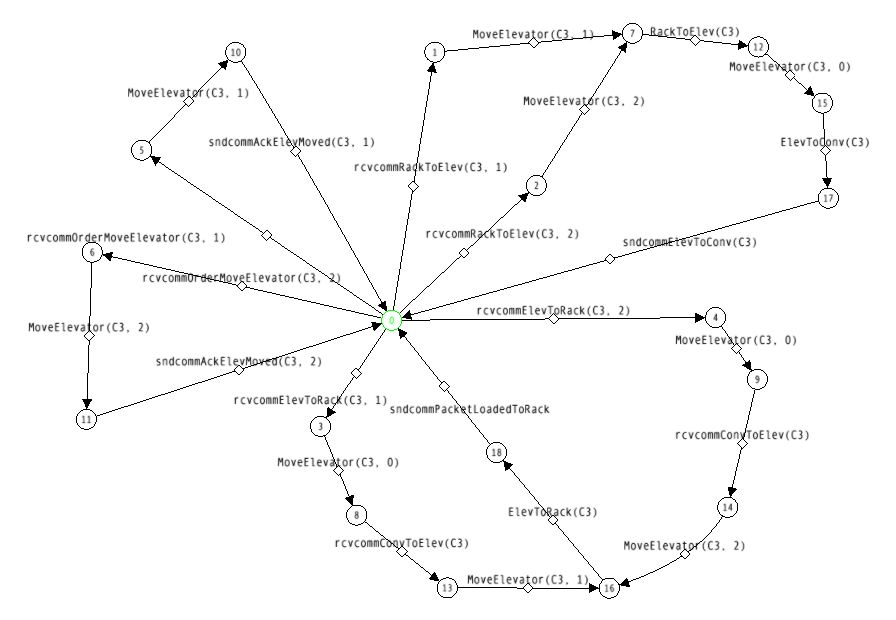
\includegraphics[width=0.7\textwidth]{model_C3}
\caption{Architecture of the system}
\label{fig:controller_C3}
\end{figure}


\subsection*{Controller C5}
\begin{figure}[h]
\center
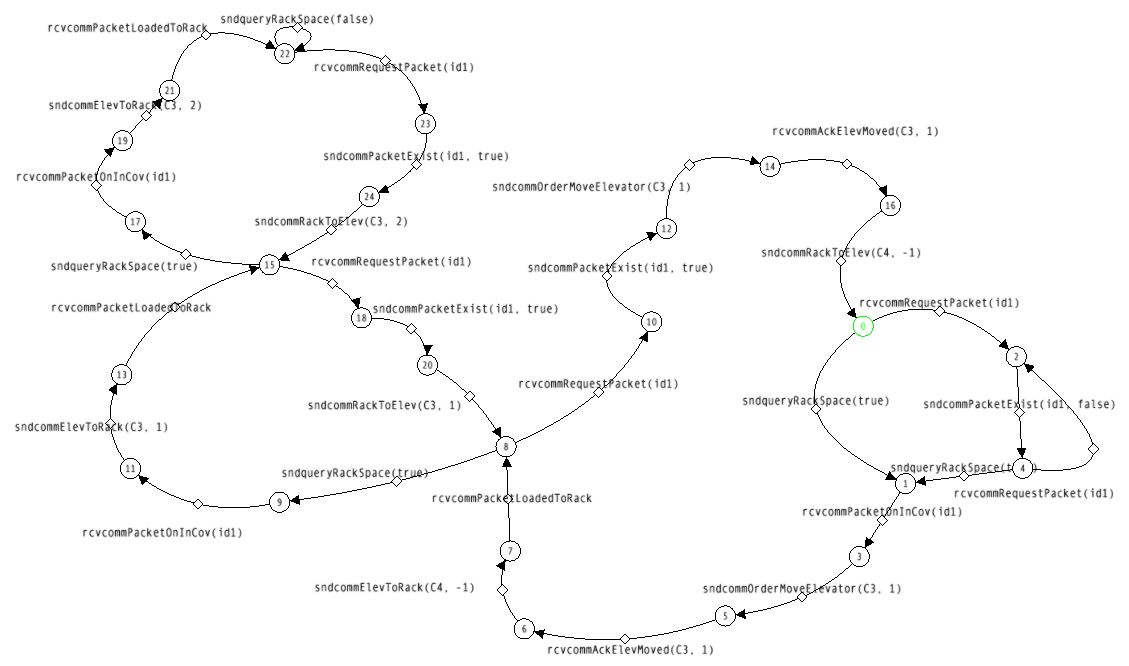
\includegraphics[width=0.7\textwidth]{model_C5}
\caption{Architecture of the system}
\label{fig:controller_C5}
\end{figure}

%
%\chapter{Verification}
%\label{chap:verification}
%\section*{Results of Verification through modal calculus formulas}
In order to check the formulae the lbs2pbes and pbes2Bool tool has been used. In addition to the global requirements, the system was checked and is verified to be \underline{deadlock free} through the formula  \textbf{[true*] $<$true$>$ true}. The results from the verification of the global requirements are presented in the following table.

The verification results for all the global requirements are listed below. \ref{tab: verification}.

\begin{table}[h]
\centering
\begin{tabular}{|l|l|l|}\hline
Requirement & Result \\\hline
1.1 & true  \\\hline
1.2 & true \\\hline
1.3.1 & true \\\hline
1.3.2 & true \\\hline
1.4 & true \\\hline
2 &  true \\\hline
3 &  true \\\hline
4.1 &  true \\\hline
4.2 &  true \\\hline
5 &  true \\\hline
6 &  true \\\hline
7 &  true \\\hline
8 &  Not verified\\\hline
9 &  true \\\hline

\end{tabular}
\caption{Verification results}
\label{tab: verification}
\end{table}

\subsection*{Verification through trace scenarios}
In order to verify the behaviour of the system, in addition to the fulfillment of the global requirements, we have simulated the following scenarios by using the ``xsim`` from the LPS tool.

The figure \ref{fig:xsim1} below shows the usage of the simulation of the LPS.

\begin{figure}[h]
\center
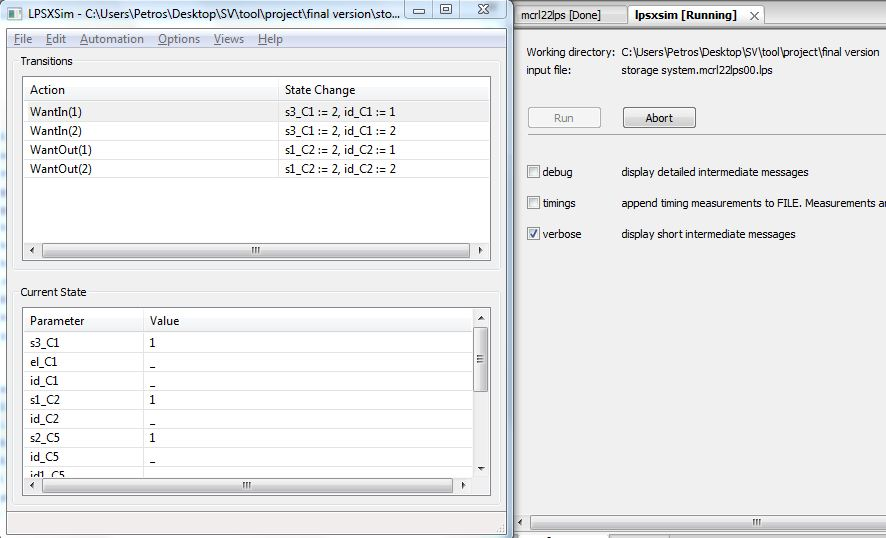
\includegraphics[width=0.8\textwidth]{xsim}
\caption{Simulation of the LPS with xsim}
\label{fig:xsim1}
\end{figure}

\begin{itemize}
\item
In this scenario, we have simulated the case that, initially a packet with “id” is inserted to the system and then another packet with same “id” is tried to be inserted into the system. The simulation results in a case that the second package is rejected \textbf{(CheckSameID.trc)}.

\item  This “.trc” files simulates the case where, the packet is inserted to the system and then it is requested and removed. Moreover, it has been tried to request the packet which is already removed from the system. Naturally, this request resulted in PacketNotFound action which should be considered as expected behavior of the system\\ \textbf{(Ins\_Pckt\_Req\_Pckt\_TryToReqSamePckt\_Again.trc)}.

\item In this scenario, the case that, the packets are delivered in the same order, is simulated. Initially, two packets are inserted to the system and then packets with id ``1`` and ``2`` are requested consecutively. It can be seen that the packets are delivered in the same order \textbf{(sameorder.trc)}.
\end{itemize}

\section*{Verification through LTS}
In this part, LTS graph for the different requirements are presented. Since, the diagrams of complicated requirements produce significantly large number of states (more than 30 states), only the understandable diagrams are included in this report. In order to obtain abstract LTS diagrams, we hide all the actions which are irrelevant for the requirement that is supposed to be examined. The ltsconvert tool is used by specifying parameter as tau-star.  In order to reduce the number of states in the LTS graph, “MaxPacketID” is determined as ''1''. Note that ''maxPacketID'' refers to number of different ''id'' that system will produce.

\begin{figure}[h]
\center
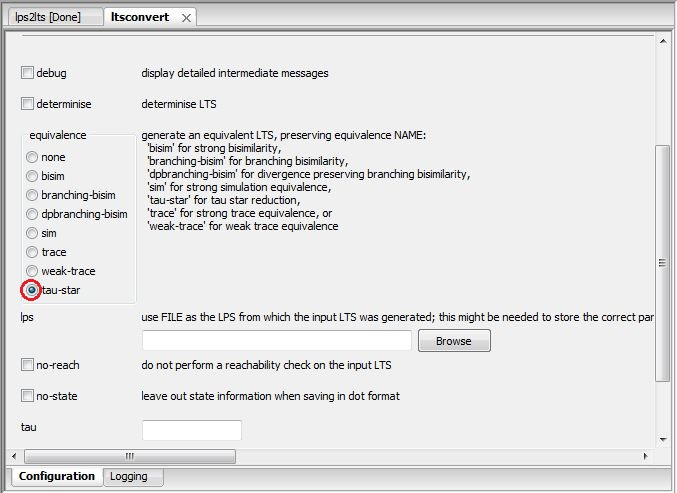
\includegraphics[width=0.8\textwidth]{ltsconvert}
\caption{LtsConvert}
\label{fig:ltsconvert}
\end{figure}

\begin{enumerate}

\item
Requirement 2:  Packet is exchanged only when the elevator platform is at the same level as that of a conveyor belt. (Figure \ref{fig:req2})

\begin{figure}[h]
\center
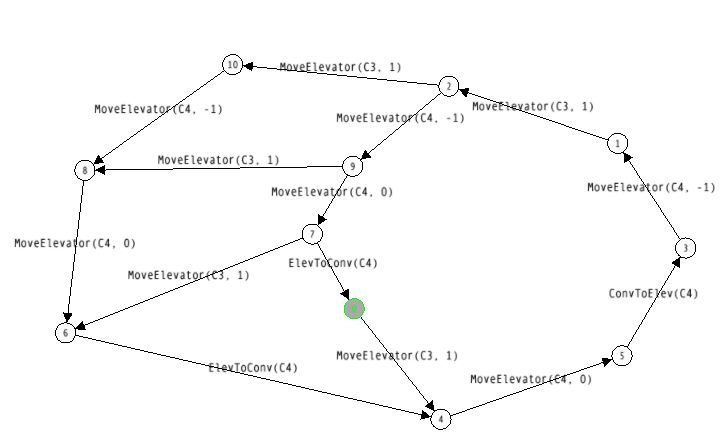
\includegraphics[width=0.8\textwidth]{req2}
\caption{Requirement 2 verification}
\label{fig:req2}
\end{figure}

In order to present the LTS with smaller number of states, all the actions other than ``MoveElevator``, ``ConvToElev`` and ``ElevToConv`` are hidden. As it was already mentioned previously in this report, the packets can be exchanged between the elevators and the conveyor belts (ConvIn and ConvOut) only in position ``0``. It is possible to observe from figure above that, C3 is moved to position ``1`` before ``MoveElevator(C4,0)`` action takes place. By considering these consecutive actions, it is possible to state that, the two elevators cannot be at same position (state 9).


\item Requirement 3: Packet is exchanged only when the elevator platform is at the same level as that of the rack.

\begin{figure}[h]
\center
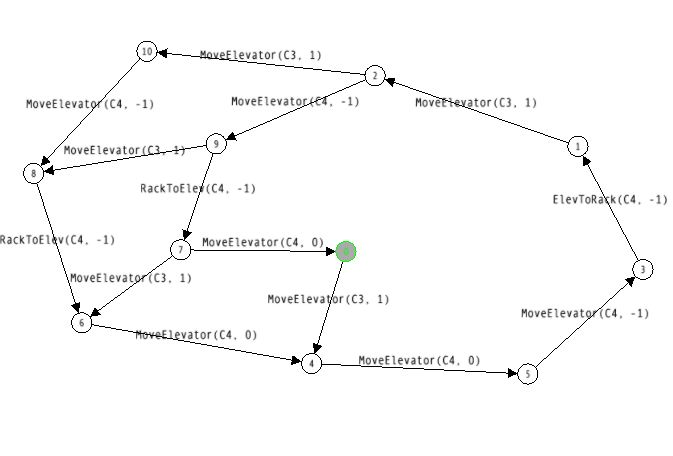
\includegraphics[width=0.8\textwidth]{req3}
\caption{Requirement 3 verification}
\label{fig:req3}
\end{figure}

The LTS graph which can be seen in figure \ref{fig:req2} is obtained by hiding all the actions other than ``MoveElevator``, ``RackToElev`` and ``ElevToRack``. In order to understand that the corresponding requirement is fulfilled or not, last MoveElevator action before RackToElev or ElevToRack is found  in the LTS graph. By using this approach, we can guarantee that the transfer of the packet is performed to the expected position successfully. The scenario that is explained in the previous sentence regarding the behavior of the RackToElev action can be observed in the following states ``10``, ``8``, ``6``, ``2``, ``9`` and ``7`` as well. Moreover, the similar behaviour for ElevToRack can be seen in states ``5``, ``3`` and ``1``. As it was mentioned before, Since the LTS graphs are obtained by using only ``1`` id, the system can accept one packet which will be transported to ``-1`` position by ``C4`` elevator.

\item Requirement 5: The lower elevator must never pass the upper one.

\begin{figure}[h]
\center
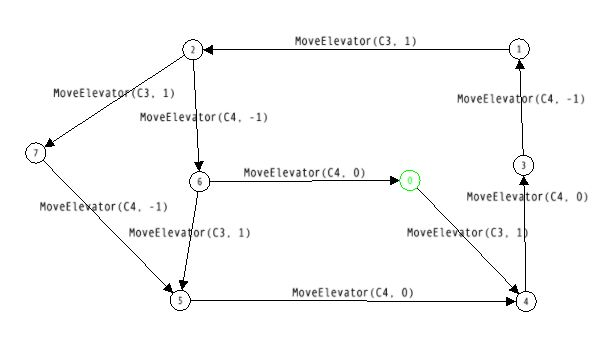
\includegraphics[width=0.8\textwidth]{req5}
\caption{Requirement 5 verification}
\label{fig:req5}
\end{figure}

In order to present the LTS all the actions except MoveElevator are hidden. This is seen in figure \ref{fig:req5} In order to specify that this requirement is verified, there should not be any path which includes MoveElevator(C3, x) action and MoveElevator(C4, y) with y > x. One may find the situation that is explained by tracking the states from the initial state. Having two or more than two ``id`` would make the state space too large to have included in this report; limiting this requirement to a single ``id``  can still be adequately described.


\end{enumerate}

\section*{Conclusions}
In this project, we learnt to work with the mCRL2 code, verification tools and analysing complex LTS graphs and ways to interpret it in simpler ways using the tool. In the end, the efforts were fruitful. All but one requirement was verified for the designed model. The requirement that could not be fulfilled was due to not verifying the property satisfactorily due to the limitation stated in the translated requirements.
%
%\chapter{Experimental results}
%\label{chap:results}
%\input{chapters/results.tex}
%
%\chapter{Conclusions and recommendations}
%\label{chap:conclusion}
%%what worked, what didn't
%recommendations: don't make our mistakes on ... bla bla bla


%\addcontentsline{toc}{chapter}{Bibliography}
%\bibliographystyle{plain}
%\bibliography{bibliography/all}
%
%\appendix
%
%\chapter{Source Code Structure}
%\label{appen:codestructure}
%%mcrl2 source code structure and code.

\end{document}
